\chapter{三大抽样分布}
\begin{introduction}
	\item Prob $\&$ Stat\quad 5.4
\end{introduction}
在本讲中,我们会给出正态分布总体下样本均值与样本方差的分布,并为之后在估计和检验任务中所需要的统计量做准备。本讲的内容可以参考图\ref{fig:lect16_framework}
\begin{figure}[ht]
\centering
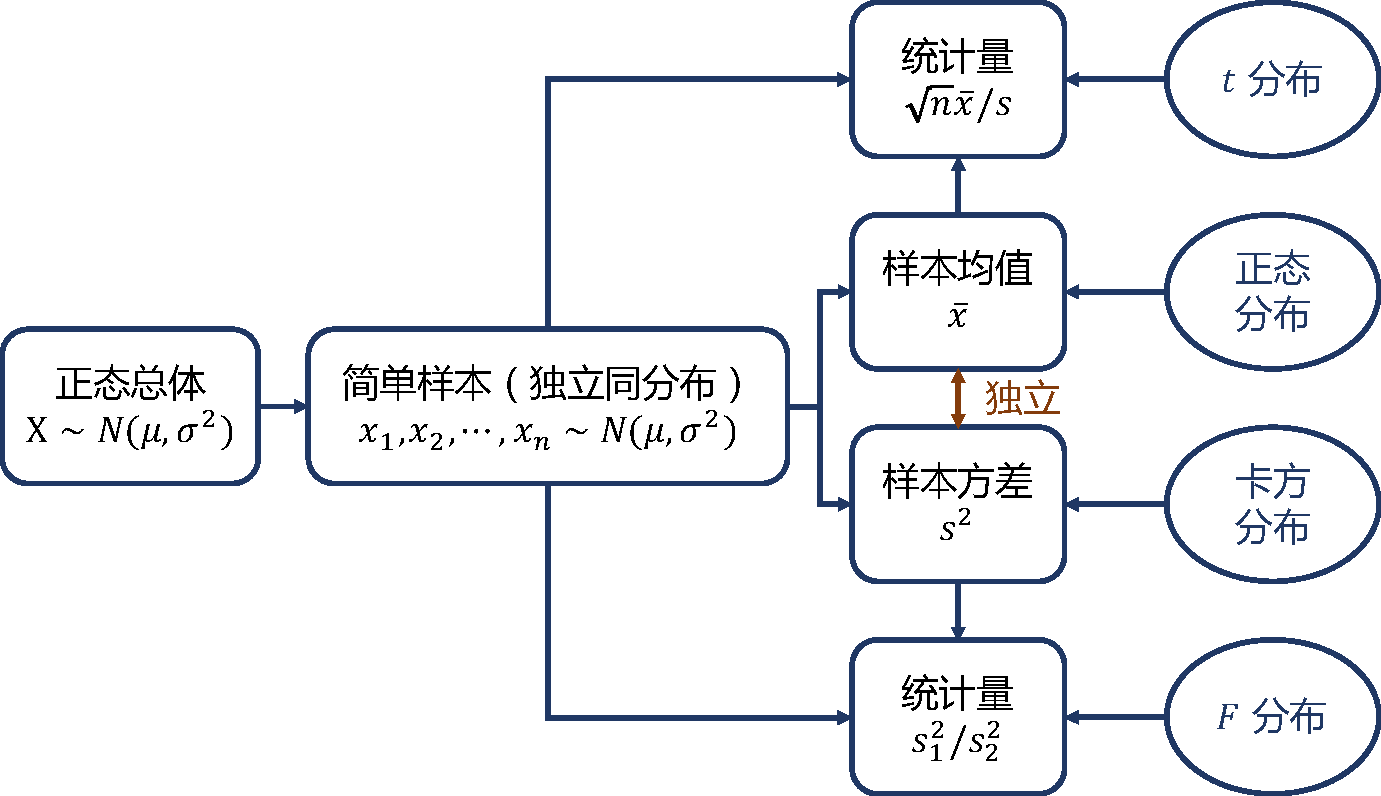
\includegraphics[scale=0.5]{image/Lect16_relation_of_distributions_from_normality.pdf}
\caption{本讲内容框架}\label{fig:lect16_framework}
\end{figure}
\section{引导问题}
在本课程中,总是存在一个假定——总体分布是正态分布。
对于任何一个正态分布随机变量$X\sim N(\mu,\sigma^2)$,我们已经证明了,经过标准化后的随机变量是服从标准正态分布,即
$$
\frac{X-\mu}{\sigma} \sim N(0,1).
$$
于是,对于样本量为$n$的样本(数据)$x_1,x_2,\cdots,x_n $均是独立同分布的,总体分布假定为正态分布$N(\mu,\sigma^2)$。我们可以计算样本均值$\bar{x} = \frac{1}{n} \sum_{i=1}^n x_i$和样本方差$s^2 = \frac{1}{n-1}\sum_{i=1}^n  (x_i - \bar{x})^2$。显然,每一个$x_i$都是正态分布$N(\mu,\sigma^2)$的随机变量,类似于标准化,这样的统计量
$$
\frac{x_i - \bar{x}}{\sqrt{s^2}}
$$
的分布是什么?仍是正态分布吗?


\section{三种分布的构造方式}
在本讲中,首先我们介绍三种“新”的分布,这些分布都来自于用于估计和检验任务中常见的统计量。与之前学习思路不同,这些分布并不是来自于伯努利实验,也并不是通过数学推导而得的。这些分布是构造出来的,我们需要关注于这三个分布的构造方式。

\subsection{卡方分布}
在第6讲中,我们已经证明了一个命题:标准正态分布$X\sim N(0,1)$,则$X^2 \sim Ga(1/2,1/2)$。我们将$Ga(1/2,1/2)$命名为卡方分布$\chi^2(1)$。另外,在第9讲中,我们也已经证明了一个命题:伽马分布具有可加性。于是,如果$Y_1,Y_2,\cdots,Y_n$独立同分布于$Ga(1/2,1/2)$,那么$$
\sum_{i=1}^n Y_i \sim Ga(n/2,1/2).
$$
我们将$Ga(n/2,1/2)$命名为自由度为$n$的卡方分布,即$\chi^2(n)$。于是,我们可以有以下定义。
\begin{definition}
    设$X_1,X_2,\cdots,X_n$独立同分布于标准正态分布$N(0,1)$,则称
    $$
    \chi^2 = X_1^2 + X_2^2 + \cdots + X_n^2 = \sum_{i=1}^n X_i^2
    $$
    的分布为自由度为$n$的$\chi^2$分布,记为$\chi^2 \sim \chi^2(n)$。
\end{definition}
根据伽马分布的期望和方差公式,我们知道,如果$\chi^2 \sim \chi^2(n)$,那么
\begin{eqnarray*}
    E(\chi^2) &=& n\\
    \text{Var}(\chi^2) &=& 2n
\end{eqnarray*}

以下两个分布是建立在卡方分布之上。
\subsection{$F$分布}
\begin{definition}{$F$分布}
    设随机变量$X_{1}\sim \chi^{2}(m),X_{2}\sim \chi^{2}(n)$,且$X_{1}$与$X_{2}$独立,则称
    $$F=\frac{X_{1} /m }{X_{2}/n}$$
    的分布是自由度为$m$与$n$的$F$分布,记为$F(m,n)$。其中,$m$为分子自由度,$n$为分母自由度。
\end{definition}

\begin{remark}
    \begin{enumerate}
        \item 根据增补变换法,可以推导$F$的密度函数为
        $$
        p_F(y) = \frac{\Gamma\left(\frac{m+n}{2}\right) \left(\frac{m}{n}\right)^{\frac{m}{2}} }{\Gamma\left(\frac{m}{2}\right) \Gamma\left(\frac{n}{2}\right)}  y^{\frac{m}{2}-1} \left(1+\frac{m}{n}y\right)^{-\frac{m+n}{2}}, y>0.
        $$
        \item 通过图像绘制,$F$分布是一个偏态分布。
        \item 易证:若$F \sim F(m,n)$,则$1/F \sim F(n,m)$;
        \item $F$分布分布数的性质。若$F_{\alpha}(m,n)$为自由度为$m$和$n$的$F$分布分位数。于是,若存在一个随机变量$F \sim F(m,n)$,则$1/F$也是一个$F$分布随机变量,其自由度分别为$n$和$m$。所以,
        $$
        \alpha  = P\left(\frac{1}{F}\leq F_{\alpha}(n,m)\right) 
        = P\left(F \geq \frac{1}{F_{\alpha}(n,m)}\right),
        $$
        从而
        $$
        P\left( F \leq \frac{1}{F_{\alpha}(n,m)}\right) =1-\alpha.
        $$
        因此,
        $$
        F_{1-\alpha} (m,n) = \frac{1}{F_{\alpha}(n,m)}.
        $$
    \end{enumerate}
\end{remark}
\subsection{$t$分布}
\begin{definition}{$t$分布}
    设随机变量$X_1$与$X_2$独立且$X_1\sim N(0,1),X_2\sim \chi^2(n)$,则称$$t=\frac{X_{1}}{\sqrt{X_{2}/n } } $$的分布为自由度为$n$的$t$分布,记为$t\sim t(n)$。
\end{definition}
\begin{remark}
    \begin{enumerate}
        \item 根据增补变换法,可以推导$t$的密度函数为
        $$
        p_t(y) = \frac{\Gamma\left(\frac{n+1}{2} \right)}{\sqrt{n\pi}\Gamma\left(\frac{n}{2}\right)} \left(1 + \frac{y^2}{n}\right)^{-\frac{n+1}{2}}, -\infty < y < \infty.
        $$
        \item $t$分布的密度函数 vs 标准正态分布的密度函数。
        \begin{enumerate}
            \item  $t$分布的密度函数和标准正态分布的密度函数均为偶函数,形状类似。
            \item 特别当$n$比较小时,尾部概率比标准正态分布的大一些。
        \end{enumerate}
    \end{enumerate}
\end{remark}


\section{正态分布下样本方差$s^{2}$的分布}
以下定理是本课程数理统计部分中最为重要的一个定理。对于这个定理,在本课程中,我们需要掌握该定理的应用,并不需要掌握证明过程,但是这个定理的证明过程是后续课程的基础。
\begin{theorem}\label{thm:lect16_normality}
	设$x_{1},x_{2},\cdots,x_{n}$是来自正态总体$N(\mu,\sigma ^{2})$的样本,其样本均值和样本方差分别为
 $$
 \bar{x} = \frac{1}{n} \sum_{i=1}^n x_i  \quad\text{和}\quad s^2 = \frac{1}{n-1}\sum_{i=1}^n(x_i- \bar{x})^2
 $$
	则有
 \begin{enumerate}
\item $\bar{x} \sim N\left(\mu, \frac{\sigma^{2}}{n}\right) $;
\item $\frac{(n-1) s^{2}}{\sigma^{2}}=\frac{\sum\left(x_{i}-\bar{x}\right)^{2}}{\sigma^{2}} \sim \chi^{2}(n-1)$;
\item $\bar{x} $与$s^{2}$独立。
\end{enumerate}
\end{theorem}
\begin{remark}
    在正态总体的假定下,这个定理阐述了三个结论。第一,样本均值$\bar{x}$服从正态分布;第二,样本方差$s^2$与卡方分布有关;第三,样本均值$\bar{x}$和$s^2$是相互独立的。
\end{remark}
我们先来看看这个定理怎么用?我们先看两个例子,这两个例子也是这个定理的重要推论。
\begin{example}
    设$x_1,x_2,\cdots,x_n$是来自正态分布$N(\mu,\sigma^2)$的一组样本,$\bar{x}$和$s^2$分别是该样本的样本均值和样本方差,则有
$$
t = \frac{\sqrt{n}(\bar{x}-\mu)}{s} \sim t(n-1)
$$
\end{example}
\begin{solution}
    根据定理\ref{thm:lect16_normality},我们可以知道,
    $$
    \frac{\bar{x}-\mu}{\sqrt{\sigma^2/n}}\sim N(0,1),\quad \text{且} \frac{(n-1)s^2}{\sigma^2} \sim \chi^2(n-1)
    $$
    而且这两者是相互独立的。所以,
    $$
    t = \frac{\sqrt{n}(\bar{x}-\mu)}{s} = \frac{\frac{\bar{x}-\mu}{\sqrt{\sigma^2/n}}}{\sqrt{\frac{(n-1)s^2}{\sigma^2}/(n-1)}} \sim t(n-1).
     $$
\end{solution}

\begin{example}
    设$x_1,x_2,\cdots,x_m$是来自$N(\mu_1,\sigma^2_1)$的样本,$y_1,y_2,\cdots,y_n$是来自$N(\mu_2,\sigma^2_2)$的样本,且两样本相互独立,记
$$
s_1^2 = \frac{1}{m-1}\sum_{i=1}^m (x_i-\bar{x})^2 \quad \text{和}\quad 
s_2^2 = \frac{1}{n-1}\sum_{i=1}^n (y_i-\bar{y})^2,
$$
其中,$\bar{x} = m^{-1}\sum_{i=1}^m x_i$ 和$\bar{y}=n^{-1}\sum_{i=1}^n y_i$,则有
$$
F = \frac{s_1^2 / \sigma_1^2}{s_2^2 /\sigma_2^2} \sim F(m-1,n-1).
$$
特别地,当$\sigma_1^2 = \sigma_2^2 =\sigma^2$时,并记
$$
s_w^2 = \frac{(m-1)s_1^2 + (n-1)s_2^2}{m+n -2} = \frac{\sum_{i=1}^m(x_i-\bar{x})^2 + \sum_{i=1}^n(y_i-\bar{y})^2}{m+n -2}
$$
则$$
\frac{(\bar{x} -\bar{y}) - (\mu_1 - \mu_2)}{s_w \sqrt{\frac{1}{m} + \frac{1}{n}}} \sim t(m+n-2).
$$
\end{example}
\begin{solution}
    根据定理\ref{thm:lect16_normality},我们知道
    \begin{eqnarray*}
        \frac{(m-1) s_1^2}{\sigma_1^2} \sim \chi^2(m-1)\\
         \frac{(n-1) s_2^2}{\sigma_2^2} \sim \chi^2(n-1)
    \end{eqnarray*}
    因为两个样本是相互独立的,所以
    $$
    F = \frac{s_1^2/\sigma_1^2}{s_2^2/\sigma_2^2} = \frac{\frac{(m-1) s_1^2}{\sigma_1^2}/(m-1)}{\frac{(n-1) s_2^2}{\sigma_2^2}/(n-1)} \sim F(m-1,n-1).
    $$
    当$\sigma_1^2=\sigma_2^2 =\sigma^2$,则$s_1^2/s_2^2 \sim F(m-1,n-1)$。根据定理\ref{thm:lect16_normality},我们知道
    $$
    (\bar{x}-\bar{y}) \sim N((\mu_1 - \mu_2),\sigma^2/m + \sigma^2/n)
    $$
    因为
    $$
   (m+n-2) s_w^2 =  (m-1)s_1^2 + (n-1)s_2^2 = \sum_{i=1}^m(x_i-\bar{x})^2 + \sum_{i=1}^n(y_i-\bar{y})^2
    $$
    可以看作两个独立的卡方随机变量的和,所以其仍为卡方分布,即$s_w^2 \sim \chi^2((m-1)+(n-1))$。且$\bar{x} - \bar{y}$与$s_w^2$是相互独立的。于是,
    $$
    \frac{(\bar{x} -\bar{y}) - (\mu_1 - \mu_2)}{s_w \sqrt{\frac{1}{m} + \frac{1}{n}}} = \frac{\frac{(\bar{x} -\bar{y}) - (\mu_1 - \mu_2)}{ \sqrt{\sigma^2\left(\frac{1}{m} + \frac{1}{n}\right)}} }{\sqrt{\frac{(m+n-2) s_w^2}{\sigma^2}/(m+n-2)}}
    \sim t(m+n-2)$$ 
\end{solution}

接下来,我们给出定理\ref{thm:lect16_normality}的证明。整体证明思路与教材中的证明思路一致,这里需要用到一些数学知识,这里我们用引理的方式罗列一下。
\begin{lemma}
  如果$\bm{A}$是一个正交矩阵,则
        \begin{enumerate}
            \item $\bm{A}$的逆矩阵等于其转置矩阵,即$\bm{A}^{-1} = A'$;
            \item $\bm{A}$的行列式为$\pm 1$。
        \end{enumerate}
\end{lemma}

\begin{proof}
我们可以构建一个$n$维随机向量$$
\bm{x} = (x_1,x_2,\cdots,x_n)' \sim N(\mu \bm{1}_n,\sigma^2 \bm{I}_n),
$$
其中$\bm{1}_n = (1,1,\cdots,1)'$一个$n\times 1$向量,且元素均为1;$\bm{I}_n$是单位矩阵,即其主对角线上的元素为1,而非主对角线上的元素为0。于是,$\bm{x} = (x_1,x_2,\cdots,x_n)'$的密度函数为
$$
p(\bm{x}) = (2\pi)^{-n/2}  |\sigma^2\bm{I}_n|^{-1/2} \exp\left\{-\frac{1}{2} (\bm{x}-\mu \bm{1}_n)' (\sigma^2 \bm{I}_n)^{-1} (\bm{x}-\mu \bm{1}_n)\right\}.
$$
接下来,我们构造一个\textbf{特别}的正交矩阵$A$,即
$$\bm{A}=\left(\begin{array}{ccccc}
	\frac{1}{\sqrt{n}} & \frac{1}{\sqrt{n}} & \frac{1}{\sqrt{n}} & \cdots & \frac{1}{\sqrt{n}} \\
	\frac{1}{\sqrt{2 \times 1}} & -\frac{1}{\sqrt{2 \times 1}} & 0 & \cdots & 0 \\
	\frac{1}{\sqrt{3 \times 2}} & \frac{1}{\sqrt{3 \times 2}} & -\frac{2}{\sqrt{3 \times 2}} & \cdots & 0 \\
	\vdots & \vdots & \vdots & \ddots & \vdots \\
	\frac{1}{\sqrt{n \times(n-1)}} & \frac{1}{\sqrt{n \times(n-1)}} &\frac{1}{\sqrt{n \times(n-1)}}& \cdots & -\frac{n-1}{\sqrt{n \times(n-1)}}
\end{array}\right)$$
并令$$\bm{y} = \bm{A} \bm{x}.$$
构造$A$的目的是为了将$\bar{x}$和$x_2-\bar{x},\cdots,x_n - \bar{x}$构成一些新的随机变量,从而可以通过变量变换法得到我们想要求的统计量的分布。这个$A$的构造方法不为一,这里提供了一个相对容易的证明方案。基于矩阵$\bm{A}$,我们发现
\begin{enumerate}
    \item $\frac{1}{\sqrt{n}} \sum_{i=1}^n x_i = y_1$,即$\bar{x} = \frac{1}{\sqrt{n}}y_1$;
    \item $\sum_{i=1}^n y_i^2 = \bm{y}'\bm{y} = (\bm{A}\bm{x})'(\bm{A}\bm{x}) = \bm{x}'(\bm{A}'\bm{A})\bm{x} = \bm{x}'\bm{x} = \sum_{i=1}^n x_i^2$。
\end{enumerate}
于是,
$$
\sum_{i=1}^n x_i^2= \sum_{i=1}^n y_i^2 = y_1^2 + \sum_{i=2}^n y_i^2 = n (\bar{x})^2 + \sum_{i=2}^n y_i^2,
$$
则$$
\sum_{i=2}^n y_i^2 = \sum_{i=1}^n x_i^2 - n(\bar{x})^2 = \sum_{i=1}^n (x_i -\bar{x})^2 = (n-1) s^2.
$$
所以, $\bm{y}=(y_1,y_2,\cdots,y_n)'$的密度函数为
\begin{eqnarray*}
p(\bm{y}) &=& (2\pi)^{-n/2} |\sigma^2 \bm{I}_n|^{-1/2} \exp\left\{-\frac{1}{2} (\bm{A}^{-1}\bm{y}-\mu \bm{1}_n)' (\sigma^2 \bm{I}_n)^{-1} (\bm{A}^{-1}\bm{y}-\mu \bm{1}_n)\right\} \cdot ||\bm{A}||\\
&=& (2\pi)^{-n/2} |\sigma^2 \bm{I}_n|^{-1/(2\sigma^2)} \exp\left\{-\frac{1}{2} (\bm{y}- \bm{A}\mu \bm{1}_n)' \bm{A} ( \bm{I}_n)^{-1} \bm{A}'(\bm{y}-\bm{A}\mu \bm{1}_n)\right\}\\
&=& (2\pi)^{-n/2} |\sigma^2 \bm{I}_n|^{-1/(2\sigma^2)} \exp\left\{-\frac{1}{2} (\bm{y}- \mu\bm{A} \bm{1}_n)' (\bm{A}\bm{A}')^{-1}(\bm{y}- \mu \bm{A} \bm{1}_n)\right\}
\end{eqnarray*}
这表明了$\bm{y}$仍服从$n$维正态分布,其均值向量为$\mu\bm{A} \bm{1}_n$,而方差-协方差矩阵为$\sigma^2 \bm{A}\bm{A}'$。
这里我们具体地讨论一下均值向量
$$
\bm{A}\cdot \mu \bm{1}_n = \mu \bm{A}\bm{1}_n = \begin{pmatrix}
    \sqrt{n}\mu\\0\\\vdots\\0
\end{pmatrix}
$$
而方差-协方差矩阵为
$$
\sigma^2 \bm{A}\bm{A}'= \sigma^2 \bm{I}_n =  \begin{pmatrix}
    \sigma^2 & 0 & 0 & \cdots & 0 \\
   0& \sigma^2  & 0 & \cdots & 0 \\
   0&  0 &\sigma^2   & \cdots & 0 \\
   \vdots & \vdots & \vdots &&\vdots\\
    0&  0  & 0  & \cdots &\sigma^2 
\end{pmatrix}
$$
这表明了$\bm{y}=(y_1,y_2,\cdots,y_n)'$中每个随机变量均是独立的,且$y_1\sim N(\sqrt{n}\mu,\sigma^2)$,而剩余的每一个分量$y_i^2 \sim N(0,\sigma^2),i=2,3,\cdots,n$。
所以,样本均值
$$
\bar{x} = \frac{1}{\sqrt{n}} y_1 \sim N(\mu,\sigma^2),
$$
而样本方差
$$
\frac{(n-1)s^2}{\sigma^2} = \frac{\sum_{i=2}^n y_i^2}{\sigma^2} \sim \chi^2(n-1), 
$$
同时,$\bar{x}$仅由$y_1$构造而得,$s^2$由$y_2,\cdots,y_n$构造而得,于是,$\bar{x}$和$s^2$是独立的。
\end{proof}

\begin{remark}
表\ref{tab_lect16_1}中列出了在正态总体下常见统计量的抽样分布及其分位数的记号。
\begin{table}[ht]
\centering
\caption{几种抽样分布及其分位数}\label{tab_lect16_1}
\begin{tabular}{cc}
\hline
分布 & $\alpha$分位数\\
\hline
$N(0,1)$ & $z_{\alpha}$\\
$\chi^2(n)$ & $\chi_{\alpha}^2(n)$\\
$F(m,n)$ & $F_{\alpha}(m,n)$\\
$t(n)$ & $t_{\alpha}(n)$\\
\hline
\end{tabular}
\end{table}
\end{remark}

\section{习题}
\begin{enumerate}
    \item $x_1,x_2,\cdots,x_n$是来自$N(\mu,1)$的样本,试确定最小的常数$c$使得对任意的$\mu\geq 0$有
$$P(|\bar{x}|< c) \leq \alpha. $$

\item 设随机变量$X \sim F(n,m)$,证明:
$$Z = \frac{\frac{n}{m}X}{(1+\frac{n}{m}X)}$$
服从贝塔分布,并指出其参数.

\item 设$x_1,x_2,\cdots,x_n$是来自$N(\mu_1,\sigma^2)$的样本,$y_1,y_2,\cdots,y_m$是来自$N(\mu_2,\sigma^2)$的样本,$c,d$是任意两个不为$0$的常数,证明
$$
	t =  \frac{c(\bar{x} - \mu_1) + d(\bar{y} - \mu_2)}{s_w\sqrt{\frac{c^2}{n} + \frac{d^2}{m}}} \sim t(n+m-2)
	$$
其中$s_w^2 =  \frac{(n-1)s_x^2 + (m-1)s_y^2}{n+m-2}$。
\end{enumerate}